%\clearpage
\section*{Praktilise küberkaitse e-kursus
süsteemiadministraatoritele}
\label{kokkuvõte}


\selectlanguage{estonian}
Käesolev magistritöö käsitleb praktilise küberkaitse e-kursuse loomist IT süsteemide administreerijatele. Põhiline töös lahendatav probleem on turvateadlike IT taristu teenuste administraatorite vähesus. Probleemi lahendamiseks loodi praktiline laboritöödel põhinev kursus, mis on kasutatav nii tasemeõppes kui ka täiendusõppes. Kursuse loomisel saadi sisend ettevõtluselt, riigisektorist, ülikoolidelt ja vilistlastelt.


\subsection*{Töö aktuaalsus}
Küberkaitse alase kvalifikatsiooni tõstmine lõpetajate ja juba töötavate spetsialistide seas on riigi prioriteet ja seetõttu pöördus Riigi Infosüsteemide Amet (\gls{RIA}) Eesti Infotehnoloogia Kolledži (\gls{EIK}) poole, et luua praktiline, tehniliselt kvaliteetne kursus, mis oleks rakendatav erinevates õppevormides ja ka täiendusõppes.
Lähtudes Eesti küberjulgeoleku strateegiast, kus rõhutati valdkonna ühte tugevamat nõrkust: kõrge kvalifikatsiooniga tööjõu vähesust \citep{Strategy2008} \emph{väidab autor}, et luues praktilise e-kursuse saab oskuse omandamise võimaldada \gls{EIK} lõpetajatele ja täiendusõppe kaudu juba töötavatele, varem lõpetanud spetsialistidele, ning seetõttu on antud teema riigile aktuaalne.


\subsection*{Kasutatud meetodid}
Kursuse koostamisel kasutati \gls{ADDIE} (\emph{Analysis, Design, Development, Implementation, Evaluation}) metoodikat, mis sobib e-kursuse loomiseks. Metoodika valimisel tutvuti erinevate \emph{Instuctional Design}  (\gls{ID}) meetoditega ja valiti \gls{ADDIE} mudel. Valitud mudeli rakendamisel kasutati eestis juurutatud juhendmaterjali\citep{OppeArenduskeskus2010}.  Loodud e-kursus erineb teistest Eestis kasutusel olevatest kursustest, kuna on loodud fookusega IT taristu teenuste kaitsele, kuna teised kursused on orienteeritud rünnetele.

Kasutatud \gls{ADDIE} mudel koosneb viiest etapist: analüüsi etapp, kavandamise etapp, väljatöötamise etapp, läbiviimise etapp, hindamise etapp  Joonis~\ref{figure:addie mudel} \citep{website:addie}.


\begin{figure}[H]
 \centering 
 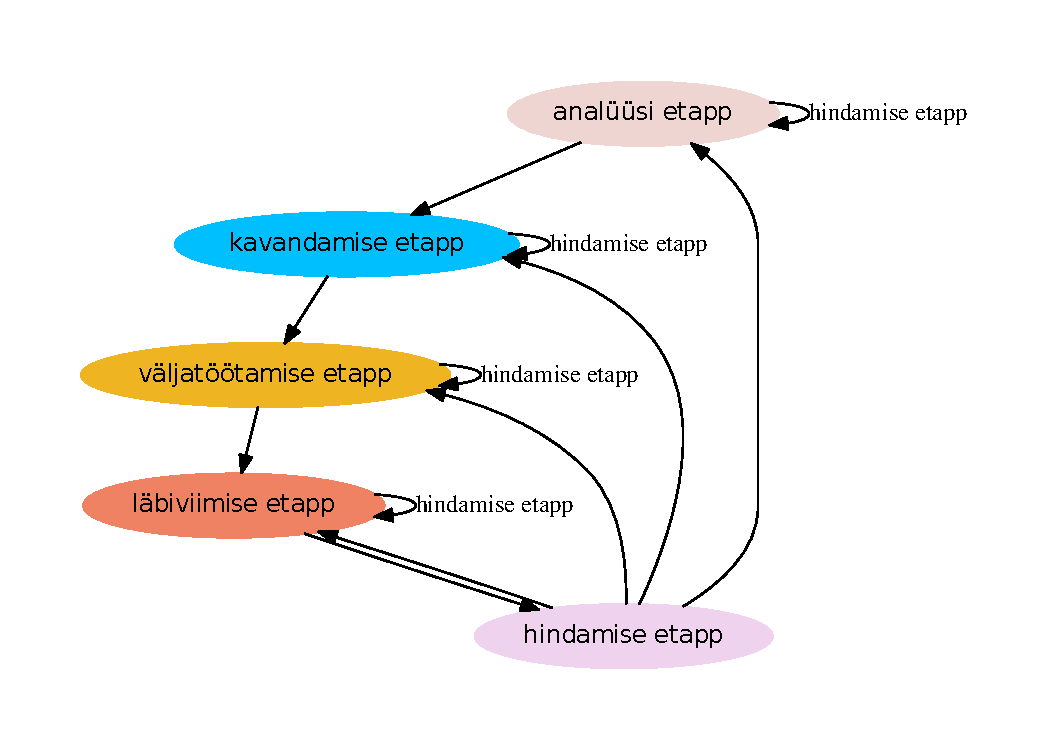
\includegraphics[width=0.6\textwidth]{addie_model_eesti.pdf}
 \rule{35em}{0.5pt} 
 \caption{ADDIE mudel} 
 \label{figure:addie mudel} 
\end{figure}

Analüüsi etapis seati eesmärgid kursusele ja määratleti õpiväljundid. Analüüsiti õppurite taset ja leiti vahe praeguse taseme ja kursuse õpiväljundite vahel, mis olid aluseks kursuse sisu planeerimisele ja teostamisele. Kavandamise etapis valiti hindamise meetodid ja kasutatav tehnoloogia -- kaugtöölaborid. Väjatöötamise etapis loodi õppematerjalid, testid, enesetestid ja kaugtöölaborite virtuaalmasinad. Lisaks varustati iga labor ja iga kursus lühikese õpijuhisega. 

Kursuse läbiviimise etapis piloteeriti kursust täiendusõppes ja tasemeõppes.

Iga eelneva etapi hindamiseks kasutati enesehindamist, õppurite ja õppejõudude tagasidet ja mõõdeti aega, mis kulus õppematerjalide omandamiseks ja laboritööde teostamiseks. Hindamise tulemusena muudeti loodud õppematerjale ja laborite ülesehitust.

Hindamise etapis mõõdeti õppuritel laboritöödele ja eesmärkide saavutamisele kuluvat aega ja jälgiti pilootgrupi koolitust, ning tehti muudatused õpijuhisesse, õppematerjali ja hulgaliselt muudatusi kaugtöölaborite süsteemi.

Kaugtöölaborite süsteemist annab hea ülevaate järgnev ettekanne "Vaba Tarkvara Päev 2014" -- "Vaba tarkvara võimalused IKT õpetamisel" \footnote{Vaba tarkvara võimalused IKT õpetamisel (Margus Ernits) 
\begin{tiny}
\url{http://www.slideshare.net/margusernits/vaba-tarkvara-vimalused-ikt-petamisel-margus-ernits-2014}
\end{tiny}
}

Kursusel kasutatakse probleemipõhist õpet praktiliste ülesannete puhul, koostööl põhinevat õpet rühmatöö vormis laboriaruannete  koostamisel ja kogukonnapõhist õpet abistavate ja selgitavate õppematerjalide loomiseks.

Antud töö käigus rakendati kaugtöölaborite süsteemi, mida muudeti vastavalt uute kursuste vajadustele. Kaugtöölaborid võimaldavad üliõpilasel teha praktilisi laboreid Internetti ühendatud arvutist ja seetõttu saab loodud kursuses suurendada praktiliste tööde mahtu, kuna kodutööd tehakse kaugtöölaborite süsteemis ja pole vajalik kooli arvutiklassis olla. 

Näiteks: e-posti turvamise laborit ei saanud varem kodutööna teha, kuna antud labori tegemiseks on vaja spetsiaalset infrastruktuuri, mida õppur ei suuda koju luua (kui suudaks, siis poleks õppuril vaja antud laborit üldse teha, kuna ta midagi juurde ei õpiks). Antud töö käigus muudetud kaugtöölaborite süsteem on nüüdseks kasutusel nelja erineva õppejõu poolt viies õppeaines, ning seda soovitakse juurutada ka teistes õppeasutustes.

Praktilise töö mahu suurendamine on üks võtmeaspektidest, mis lubavad pakkuda kvaliteetset õpet, ning kaugtöölabor annab selleks vajaliku tehnilise baasi. Kõik kaugtöölabori komponendid on loodud kasutades vaba tarkvara ja tulemus on samuti vaba tarkvara, mis on kättesaadav kõigile ja juurutatav teistes koolides ja õpet pakkuvates ettevõtetes\footnote{Kaugtöölaborite süsteemi github leht --- \url{https://github.com/magavdraakon/i-tee}}.


\subsection*{Töö tuelmused ja hinnang kasutatud metoodikale}
Töö tulemusena valmis uus väljundipõhine kursus mahuga 6 EAP-d (32h loenguid, 46h praktilist tööd, 78h iseseisvat tööd), mida piloteeriti Eesti Infotehnoloogia Kolledžis tasemeõppes ja täiendusõppes. Kursus koosneb loengutest, nende videosalvestustest, enese ja eelduste testidest, praktilistest, probleemile orienteeritud laboritöödest ja interaktiivsetest testidest.

Kursuse tagasiside on positiivne ja kursuse tulemusena paraneb tudengite ja ettevõtete süsteemide administreerijate turvateadlikus.
Kursuse loomisel kasutati erinevate ettappide kvaliteedi hindamiseks teiste õppejõudude ja tudengite abi.


Kõik kursuse käigus loodud materjalid on avalikustatud \emph{Creative Commons Attribution-ShareAlike 3.0 Unported} (\gls{CC-BY-SA}) litsentsi alusel, tagamaks kursuse maksimaalset mõju Eesti õppeasutustes. Lisaks aitab avalik õppematerjal täiendusõppe võimalikul õppuril otsustada, kas loodud kursus vastab tehama teadmistele ja vajadustele.
 
Autori roll seisnes nõuete ja õpiväljundite loomises, laboritööde ja loengumaterjalide koostamises koostöös teiste õppejõududega (panus >90\%) ja kursuse piloteerimises nii taseme- kui täiendõppes.

Autori hinnangul on kasutatud metoodika (\gls{ADDIE} ja kaugtöölaborite süsteem) sobiv, kuna loodud lahendus on kasutatav õppetöös ja täiendusõppes, ning kursuse loomisel arvestati sihtrühmaga ja hinnati iga etapi puhul loodu sobivust eesmärkidega. Kaugtöölaborite kasutamine võimaldas suurendada praktilise töö mahtu ja on paremini suuratud oskuste ja kvalifikatsiooni omandamisele, võrreldes loengute/praktikumide ja kodutööna antava kodulugemisega.


\subsection*{Edasised arengud peale lõputöö kaitsmist}
Peale kursuse loomist on seda kasutatud kolm õppejõudu ja antud kursust juurutatakse ka Kaitseväe küberlaboris. Kursus õnnestus ja autor sai õppejõuna suurepärase tagasiside õppuritelt, ning autor valiti Eesti Infotehnoloogia Kolledži (\gls{EIK})  aasta õppejõuks (2013/2014 õppeaastal). 
Töö tulemusena on paranenud \gls{EIK} lõpetajate kvalifikatsioon kuna kursus on kasutusel ka täiendusõppes, siis on koolitatud 322 IT spetsialisti erinevatest organisatsioonidest (september 2014.a.)

Autor jätkab kaugtöölaborite süsteemi ja praktiliste e-kursuste valdkonnas ja on juhendanud ühe magistritöö ja ühe diplomitöö antud tööst välja arendatud teemadel.

Autor jätkab küberkaitse alaste koolituste ja õppuste temaatikaga Tallinna Tehnikaülikooli doktoriõppes.
